\documentclass{article}

\usepackage[left=2.54cm,bottom=2.54cm,top=2.54cm,right=2.54cm,nohead,nofoot]{geometry}
\usepackage{listings}
\usepackage{graphicx,epsfig,latexsym,subfig}
\usepackage{amsmath,amsthm,amsfonts,amscd,amssymb,bm,mathtools,setspace,fancyhdr,commath,mathrsfs,mathtools,dsfont,tikz-cd,soul,booktabs}
\usepackage{tikz}
\usepackage{tkz-euclide}
\usetkzobj{all}
\usetikzlibrary{calc,decorations.markings}
\everymath{\displaystyle}
\usepackage{spverbatim}
\usepackage{float}

\pagestyle{empty}
\renewcommand{\headrulewidth}{2pt}
\cfoot{\thepage}
\cfoot{\vspace{0.4cm} \thepage}

\begin{document}
\bigskip
\begin{Large}\begin{center}\textbf{Report for XGBoost Algorithm}\end{center}\end{Large}
\begin{spacing}{.75}
\begin{center}\begin{Large} Xinyi Hou, Yuan Xu, Wenyu Li, Yingxi Yu \end{Large}\end{center}
\begin{center}\begin{large}Nov. 19, 2016\end{large}\end{center}
\end{spacing}
\begin{spacing}{1.5}
\begin{large}

\section{Abstract for Final Report}
    The topic of our group is selected from Kaggle and we are expected to build a recommendation system for Santander Bank. In detail, our goal is to predict which products the customer will purchase in the next month based on their pasting 1.5 year behaviors data and that of similar customers. To solve this problem, we use four different machine learning methods: logistic regression, SVM, random forest and XGBoost. Since the data size is large and there is no clear response variable in the training set, different subteams use different subsets of the original training set and build their own response variable. What is more, every subteams drop some useless variables and simplify the training set. It is difficult to compare the four different methods, because every subteams manipulate the data in their own way. The logistic regression and SVM subteams both build 24 classifiers for 24 products and the accuracy is high, which is above 0.9. However, we cannot say these two classifiers are powerful, because the training set is quite unbalanced. The random forest and XGboost both build only one multi-classifier model. The accuracy for these two are 0.90 and 0.63. As these two subteams use different data cleaning method and response variable, we cannot say random forest is better than XGboost. In summary, all four methods could provide reasonable predictions and this would help the Santander Bank to build a more effective recommendation system.

\section{Methods}

\noindent \indent XGBoost is short for ``Extreme Gradient Boosting” and is widely used in machine learning problems, especially classification problems with good results in most cases [1][2]. The idea behind is very simple. Firstly, we only have one weak classifier, one decision tree. During each iteration, we would add a tree, eventually, XGBoost method makes our model grows to be an ensemble tree. Examples that are mis-classified before gain weight and examples that are classified correctly lose weight. The goal is to minimize the loss function, which takes into account the error and the complexity of the ensemble tree.

\subsection{Data Pre-processing}

\noindent \indent Since there are many missing values and outliers, the first thing is to clean data. 27334 records with 9 consecutive NA values are deleted and the extreme values (for an instance, the 99 percent quantile of the age variable is 88 years old) are excluded. After exploring the original data, we decide to use 32 features to predict the response. The 32 features include \verb|"pais_residencia"|, \verb|"age"|, \verb|"ind_nuevo"|, \verb|"antiguedad"|, \verb|"ind_empleado"|, \verb|"renta"|, \verb|"ind_actividad_cliente"|, \verb|"segmento"| and 24 product status. For the \verb|"age"|, \verb|"antiguedad"| and \verb|"renta"|, we cut them into 5 intervals and they also become categorical features now. 

The response is the additional product which the customer would add in the next month. If the customer adds more than one product, we only randomly pick one of them. To make the data size smaller and the problem easier, we subset the samples with nonzero response, which means we only consider the records with additional product.

\subsection{XGBoost Algorithm}

\noindent \indent To find the best parameters given the training data. In order to do so, we need to define a so-called objective function, to measure the performance of the model given a certain set of parameters. Here for XGBoost algorithm, the objective function contains two parts: training loss and regularization.
\[
Obj(\Theta) = L(\theta) + \Omega(\theta)
\]
where $L$ is the training loss function, and $\Omega$ is the regularization term. The training loss measures how predictive our model is on training data. The regularization term controls the complexity of the model, which helps us to avoid overfitting. Here we define these two items as:
\[
L(\theta) = \sum_{i}(y_i - \hat{y_i})^2
\]
\[
\Omega(f) = \gamma T + \frac{1}{2}\lambda\sum_{j = 1}^{T}(w_j)^2
\]
 



\section{Results} 

\noindent \indent Different from some other groups, we only apply the algorithm once and fit a multi-classifier model. We randomly pick 70\% of the data to be the training data, and the rest 30\% to be the test set. By changing the main parameters [3] max.depth among 5, 6, 7, the number of trees among 10, 50, 100, and the step size among 0.1, 0.5, 1, we get the results displayed in the tables as below.
\begin{table}[h]
\centering
\caption{Accuracy for Training Data}
\label{Accuracy for Training Data}
\begin{tabular}{cccccccccc}
\hline
max.depth       & \multicolumn{3}{c}{5} & \multicolumn{3}{c}{6} & \multicolumn{3}{c}{7} \\ \hline
\# of trees     & 10    & 50    & 100   & 10  & 50       & 100  & 10    & 50    & 100   \\
step size = 0.1 & 62.06\%    & 62.45\%     & 62.79\%     & 62.32\%    & 62.77\%         & 63.10\%      & 62.54\%     & 62.89\%      & 63.24\%      \\
step size = 0.5 & 62.47\%    & 63.37\%       & 63.46\%      & 62.79\%   & 63.70\%  & 64.48\%     & 62.97\%       & 64.20\%      & 64.32\%      \\
step size = 1   &38.30\%       & 31.70\%      &35.07\%       &18.31\%     & 36.78\%         &36.65\%      &30.46\%       &46.37\%       &44.31\%       \\ \hline
\end{tabular}
\end{table}

\begin{table}[h]
\centering
\caption{Accuracy for Test Data}
\label{Accuracy for Test Data}
\begin{tabular}{cccccccccc}
\hline
max.depth       & \multicolumn{3}{c}{5} & \multicolumn{3}{c}{6} & \multicolumn{3}{c}{7} \\ \hline
\# of trees     & 10    & 50    & 100   & 10  & 50       & 100  & 10    & 50    & 100   \\
step size = 0.1 & 62.09\%      & 62.37\%     & 62.63\%      &62.30\%     & 62.59\%       & 62.80\%      & 62.45\%      & 62.76\%      & 63.10\%      \\
step size = 0.5 & 62.41\%     & 62.80\%     & 62.92\%      & 62.57\%    &62.85\%     & 62.94\%   & 62.61\%      & 62.88\%      & 62.89\%      \\
step size = 1   &38.45\%       & 31.80\%      & 35.29\%      &18.30\%     & 36.72\%         &  36.98\% &30.61\%       &46.55\%      &44.45\%     \\ \hline
\end{tabular}
\end{table}

\noindent \indent From the above tables, we can see the highest accuracy for the training set is 64.48\%, and for the test set is 62.94\%, when max.depth = 6, the number of rounds(the number of trees) = 100 and the step size = 0.5. For step size = 0.1 or 0.5, the training accuracy and test accuracy are both about 62\%, which are relatively high. When step size = 1, the accuracy for training and test set are about 40\%, which means this situation is not ideal.

\noindent \indent According to the best parameters that lead to highest test accuracy, we got the feature importance plot and final ensemble tree as below. The feature importance figure shows the different gains for different features. From the plot, we can see features \verb|"ind_cno_fin_ult1"|, \verb|"ind_recibo_ult1"| and \verb|"ind_cco_fin_ult1"| obtain the first three highest gains. As for the final ensemble tree, to save space, we just show the first three trees.

\begin{figure}[H]
\centering
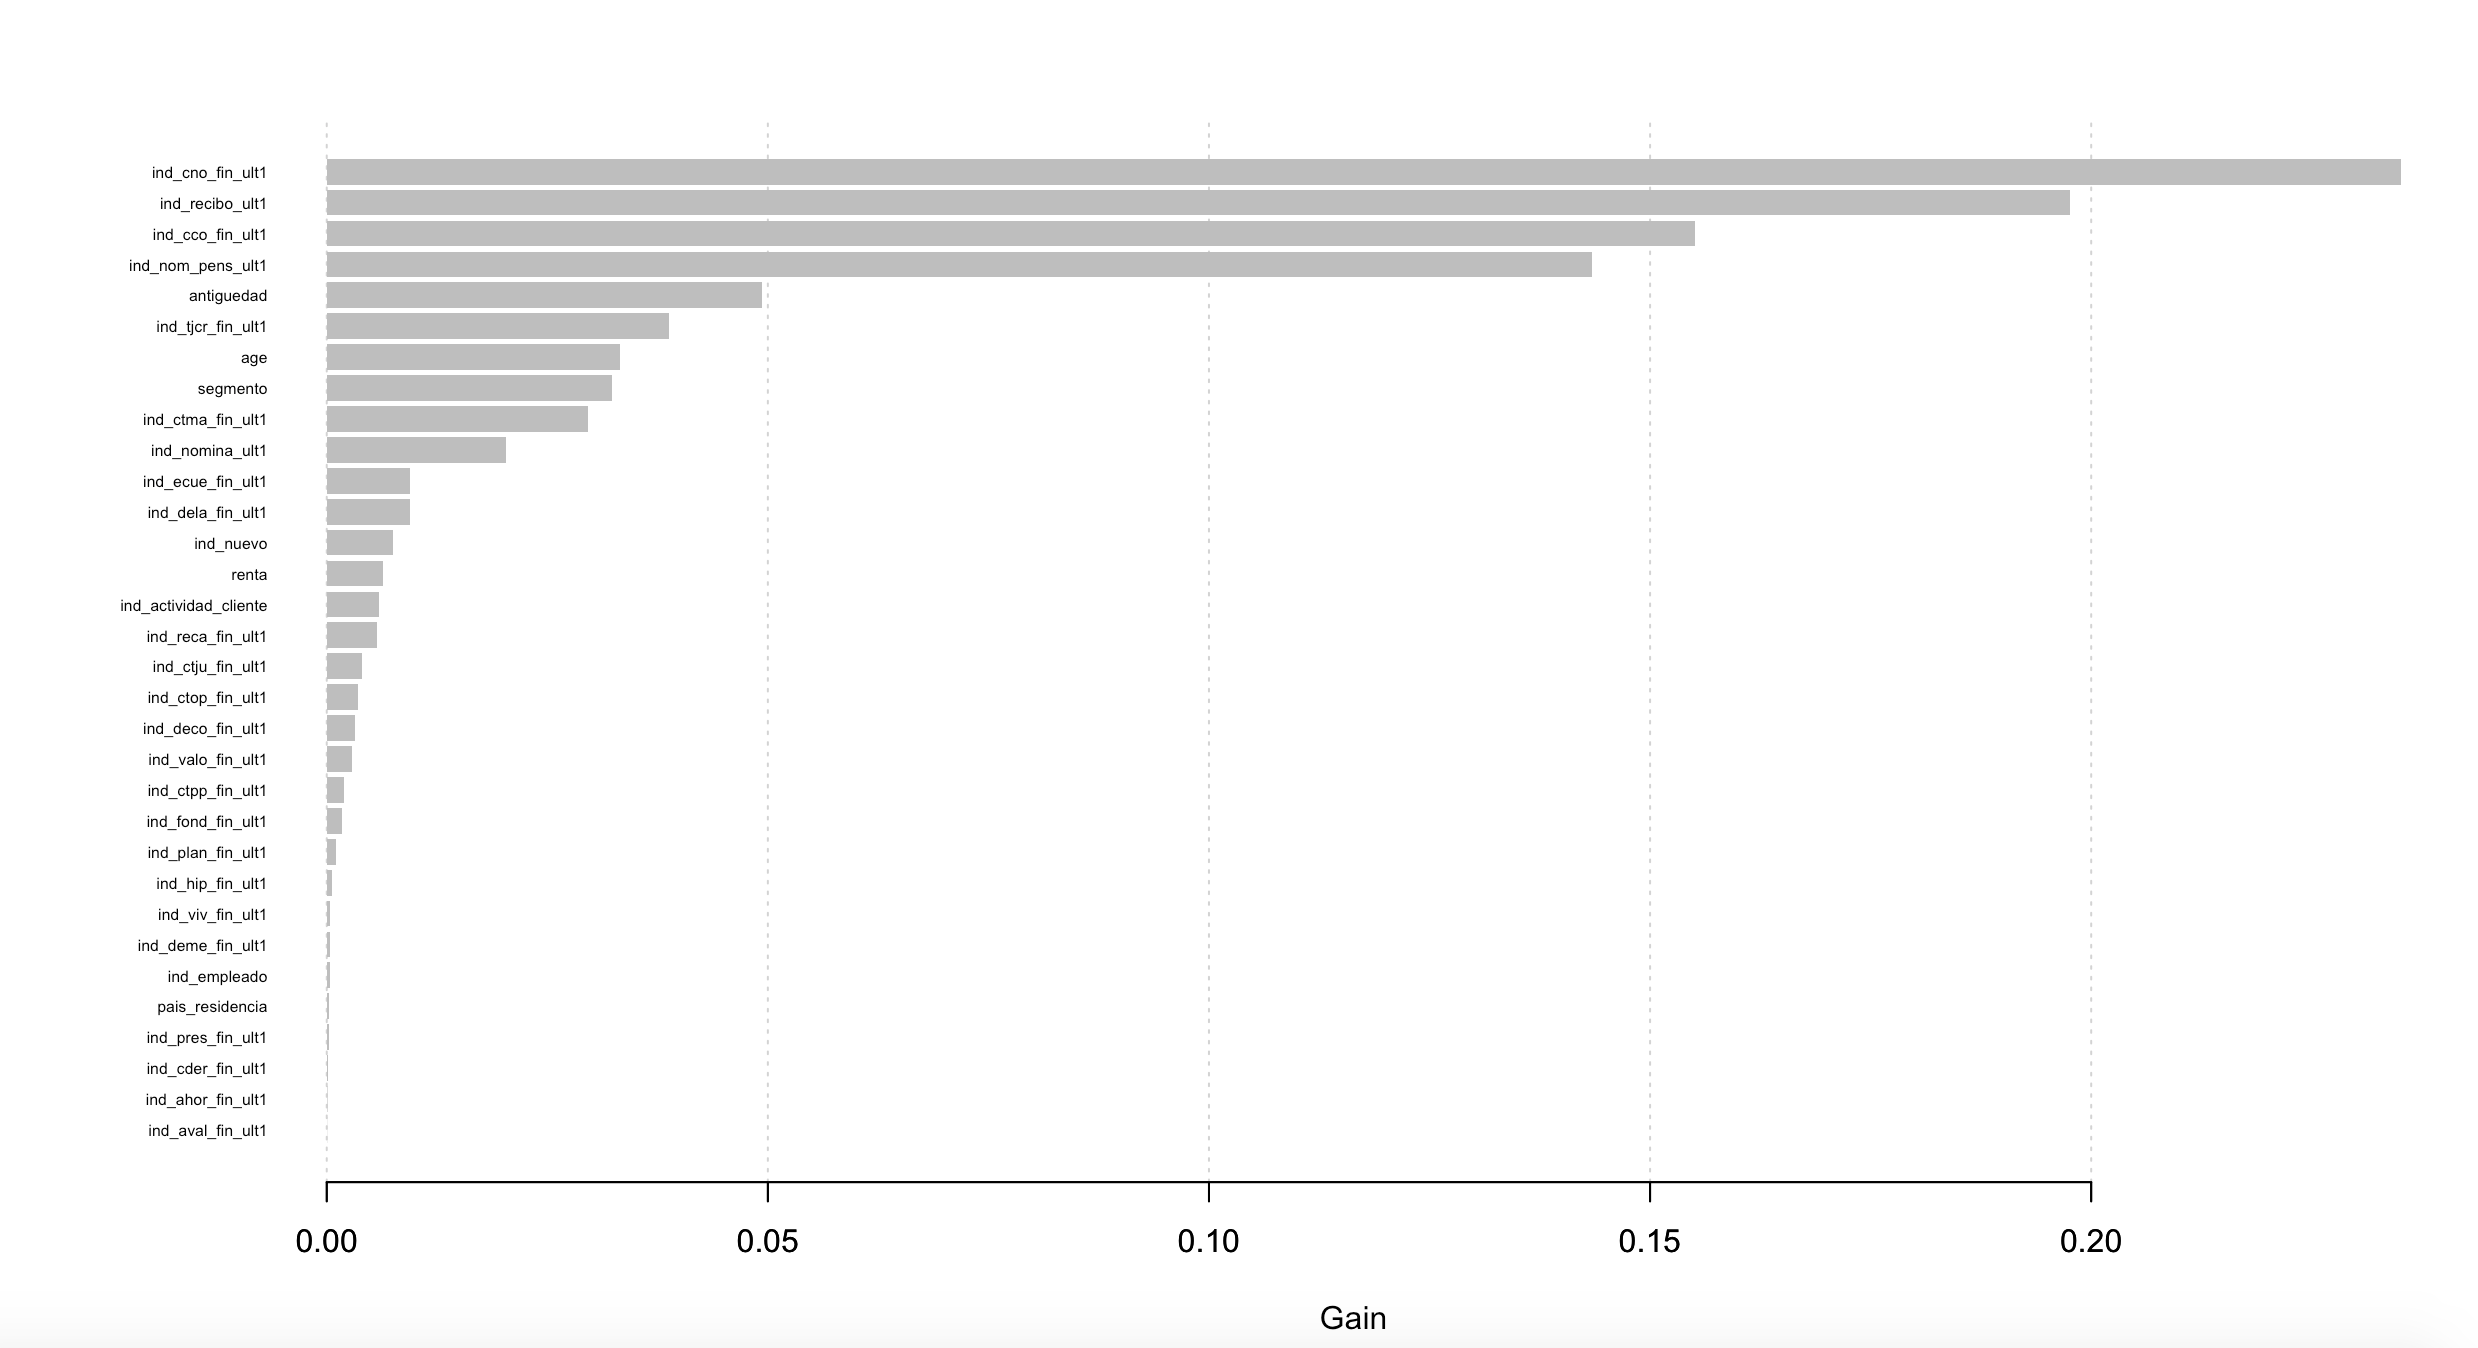
\includegraphics[width = 160mm]{113.png}
\caption{Feature Importance}
\end{figure}

\begin{figure}[H]
\centering
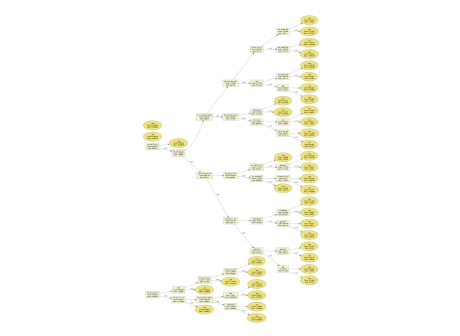
\includegraphics[width = 160mm]{12.png}

\caption{Final Ensemble Tree}
\end{figure}


\section{Discussion}

To make the model better, we could dive deeper. For example, we may consider more features and not cut some variables into intervals. We may also take the history length of the used products into account.

Due to the vague description of the problem, we are not sure how many new products to predict for each user. In fact, most members seldom tried new products based on historical records. Some valuable information might be lost since we drop some predictors and only pick one new product every time (if more than one).


\section{Author Contribution}

This subgroup consists of fours members, Xinyi Hou, Yingxi Yu, Wenyu Li, and Yuan Xu. Everyone in this subgroup gathered together to discuss how to tackle the problem, determine the method and tune parameters. More specifically, Xinyi was the leader of the whole big project group, pre-processed the data and wrote the abstract of the overall report; Yingxi wrote the initial model code and made the popwerpoint; Wenyu participated in initial model code writing and completed the report; and Yuan mainly focused on the report.

\begin{thebibliography}{9}

\bibitem{1}
  Tianqi Chen, Carlos Guestrin
  \emph{XGBoost: A Scalable Tree Boosting System}. Preprint.

\bibitem{2}
  \emph{Awesome XGBoost}.
  https://github.com/dmlc/xgboost/tree/master/demo
  
\bibitem{3}
  \emph{XGBoost Parameters}.
  http://xgboost.readthedocs.io/en/latest//parameter.html



\end{thebibliography}


\end{large}
\end{spacing}
\end{document}
